\documentclass{article}
\usepackage[utf8]{inputenc}
\usepackage{tikz}
\usepackage{graphicx}
\usepackage{hyperref}
\title{\textbf{BINARY HALF SUBTRACTOR}}
\author{Vallabhaneni Rupa Sai Sreshta}
\begin{document}
\maketitle
\begin{tableofcontents}
\begin{abstract}
This manual shows how to execute Binary-half-Subtractor having two inputs A and B.
\end{abstract}
\section{COMPONENTS}
\begin{tabular}{|c||c||c|}
\hline
\textbf{component} & {value} & {quantity} \\
\hline
 \textbf{Breadboard}  &  &  1  \\
 \hline
 \textbf{Resistor}  & {220ohm} & {1} \\
 \hline
 \textbf{Arduino} & {Uno} & 1\\
 \hline
 \textbf{Sevensegment display} & {Common anode} & {1}\\
 \hline
 \textbf{Jumper wires} &   &  {20}\\
 \hline
\end{tabular}
%\centering{\textbf{Table}}
\\
\section{BINARY HALF SUBTRACTOR WITH TWO INPUTS}
Half subtractor is a combination circuit with two inputs and two outputs which is difference and borrow. It produces the difference between the two binary bits at the input and also produces an output (Borrow) to indicate if a 1 has been borrowed. In the subtraction (A-B), A is called a Minuend bit and B is called as Subtrahend bit.
\newline
\\
%\begin{center}
%\begin{tikzpicture}
%\draw[ultra thick] (0,0) -- (0,3)
%\end{tikzpicture}
%\end{center}

\centering
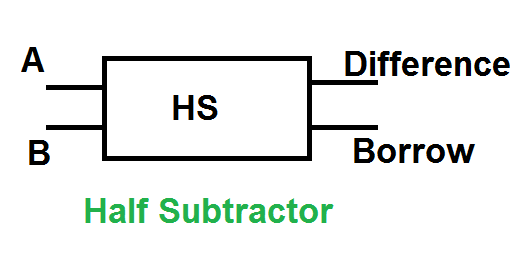
\includegraphics[scale=0.5]{bhs.png} 
\\


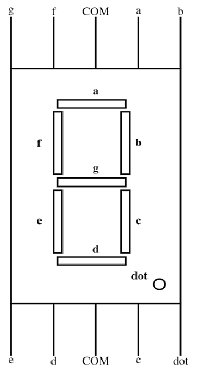
\includegraphics[scale=1.5]{sevenseg.png}
%\centering
\\
%\textbf{Connections :-}
%\vspace{0.3cm}
%\begin{tabular}{|c|c|c|}
%\hline
%\textbf{Arduino} & 2 & 3   \\
%\hline
%\textbf{Display} & {a} & {b}  \\
%\hline
%\end{tabular}
%\centering\textbf{Table.1}

\section{TRUTH TABLE}
\vspace{7mm}
\begin{tabular}{|c||c||c||c|}
\hline
\textbf{A} & {B} & {D} & {X}\\
\hline
\textbf{0} & {0} & {0} & {0}\\
\textbf{0} & {1} & {1} & {1}\\
\textbf{1} & {0} & {1} & {0}\\
\textbf{1} & {1} & {0} & {0}\\
\hline
\end{tabular}
\newline
\newline
\newline
\textbf{Equations :-}
\newline
\newline
Equation for D is
\begin{equation}
D= A'B+AB'
\end{equation}
Equation for X is
\begin{equation}
X=A'B
\end{equation}
\\
\begin{tabular}{|c|c|c|}
\hline
\textbf{Arduino} & 2 & 3  \\
\hline
\textbf{Display} & {a} & {b}  \\
\hline
\end{tabular}
\\
\centering
\textbf{Table-1}
\centering
\\
\textbf{Problem:}
Make the connections as per Table-1 and execute the following program.
\end{tableofcontents}
\\
\vspace{1cm}
\href{https://github.com/RupaSaiSreshta/FWC/blob/main/Assignment1-IDE/Code/src/main.cpp}{https://github.com/RupaSaiSreshta/FWC/blob/main/Assignment1-IDE/Code/src/main.cpp}
\end{document}
